
\section{Experiment}
\label{cp3:experiment}









\begin{landscape}
    \begin{figure}
        \centering
        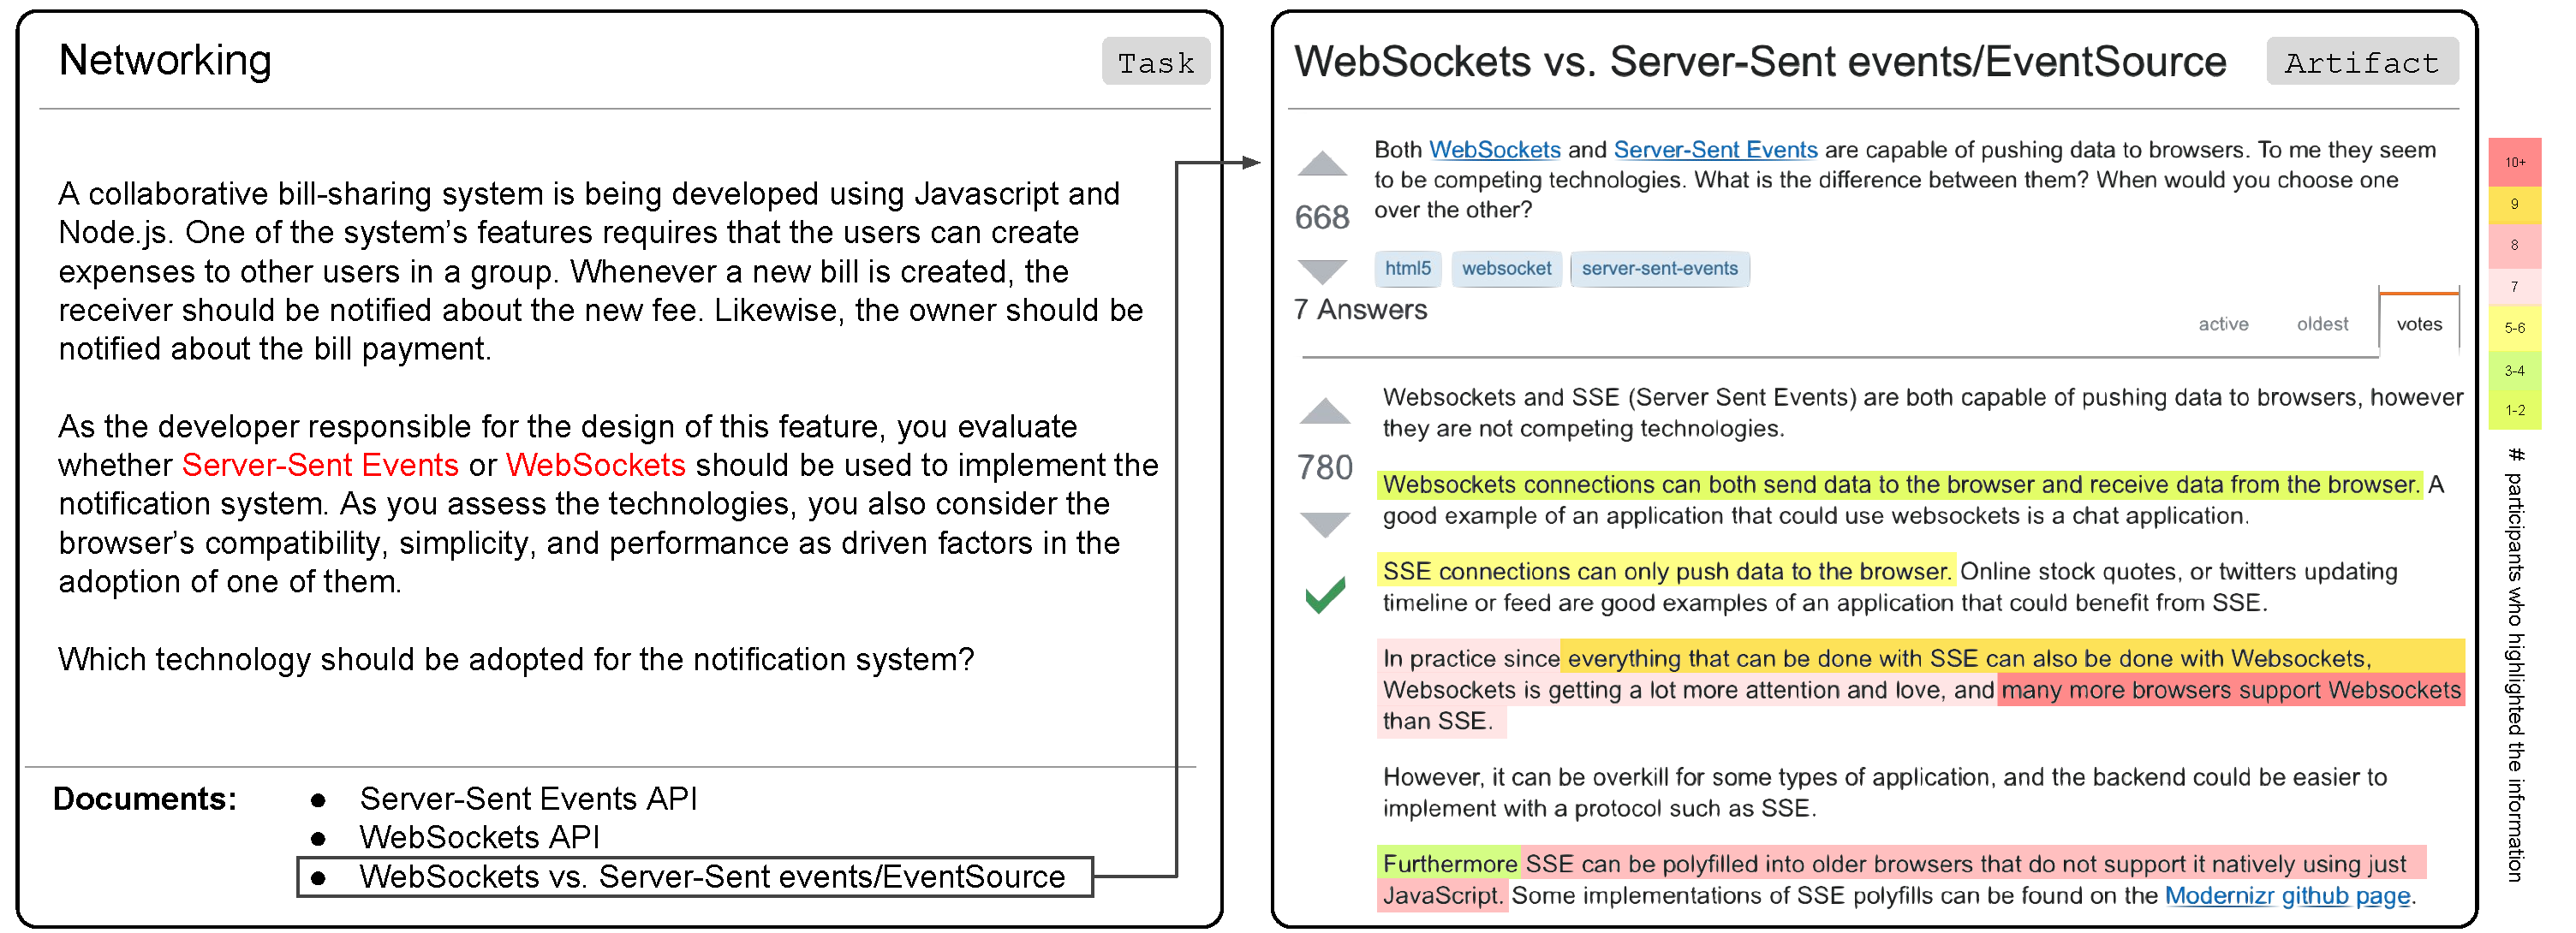
\includegraphics[width=\dimexpr\linewidth-4\fboxsep-2\fboxrule]{cp3/heatmap}
    \caption{An example of a task description and a depiction of collected data, shown as a heatmap of text that participants highlighted as relevant to the task; the warmer the color, the more participants highlighted the text}
    \label{fig:task-highlights-heatmap}
    \end{figure}
\end{landscape}



\begin{table}
\caption{Tasks overview}
\begin{scriptsize}
\vspace{-1mm}  


\begin{threeparttable}    
\rowcolors{2}{}{lightgray}
\begin{tabular}{ll}
\hline    
\textbf{Task} & \textbf{Description} \\ 
\hline
\hline
Bugzilla & 
\parbox[l][0.9cm][c]{11cm}{Locate information about Bugzilla's REST API custom fields and how they can be included as part of the \texttt{GET /rest/bug} payload}  \\
%
Databases & 
\parbox[l][0.9cm][c]{11cm}{Review Q\&A forums and decide between the adoption of ORM or JDBC for a system's database being migrated from C to Java}  \\ 
%
GPMDPU & 
\parbox[l][0.9cm][c]{11cm}{Locate constraints or limitations about the GPMDPU shortcuts feature in order to work in a patch for this feature}  \\
%
Lucene & 
\parbox[l][0.9cm][c]{11cm}{Review the Lucene documentation and bug reports to understand how it computes similarity scores during indexing, particularly the BM25 score function, such that you can address a change request} \\
%
Networking & 
\parbox[l][0.9cm][c]{11cm}{Review the MDN documentation and Q\&A forums to decide between the adoption of Server-sent events or WebSockets technologies for a notification system being developed using Javascript } \\ 
%
Yargs & 
\parbox[l][1.2cm][c]{11cm}{Review the Yargs documentation and bug reports to check whether the API provides support for parsing mutually exclusive arguments, which is a requirement for a command line tool being developed in Python } \\
\hline
\end{tabular}
\end{threeparttable}    
\end{scriptsize}
\smallskip
\label{tbl:tasks-overview-cp3}
\end{table}








\begin{table}
\caption{Corpus overview}
\begin{footnotesize}
\begin{center}
% \begin{threeparttable} 
\rowcolors{2}{}{lightgray}
\begin{tabular}{l|cccccccc}
\hline    
\textbf{Task} 
&  \textbf{\# participants}
&   \textbf{\# Artifacts} 
&   \textbf{API} 
&   \textbf{Bugs} 
&   \textbf{Q\&A} 
&  \textbf{\# Sentences} \\ 
\hline    
\hline
Bugzilla    & 18 & 3 & 3 & 0 & 0 & 459 \\
Databases   & 17 & 3 & 0 & 0 & 3 & 232 \\
GPMDPU      & 18 & 3 & 0 & 3 & 0 & 291 \\
Lucene      & 15 & 3 & 2 & 1 & 0 & 170 \\     
Networking  & 17 & 5 & 4 & 0 & 1 & 313 \\
Yargs       & 18 & 3 & 1 & 1 & 1 & 409 \\
\hline    
\hline 
\rowcolor{white}
Total       & 20 & 20 & 10 & 5 & 5 & 1874  \\
\hline 
\end{tabular}
% \begin{tablenotes}
% \end{tablenotes}   
% \end{threeparttable} 
\end{center}
\end{footnotesize}
\label{tbl:corpus-stats}
\end{table}




\begin{figure}
\begin{mdframed}[backgroundcolor=gray!15] 
\begin{scriptsize}

\noindent On a scale of 1 to 5, how familiar are you with the task's technologies: \smallskip

\quad \textit{(not at all familiar)} ~$1$ - $2$ - $3$ - $4$ - $5$ ~\textit{(extremely familiar)} 

\noindent\rule{8cm}{0.4pt} \smallskip

\noindent On a scale of 1 to 5, what was the level of difficulty of the task: \smallskip

\quad \textit{(very easy)} ~$1$ - $2$ - $3$ - $4$ - $5$ ~\textit{(very hard)} 

\noindent\rule{8cm}{0.4pt} \smallskip

\noindent Please evaluate the following sentences and mark only correct statements: \smallskip

\noindent $\square$ SSE are bidirectional and it can be used for pushing notifications to the bill-sharing system; \smallskip

\noindent $\square$ SSE works over HTTP with no additional components; \smallskip
    
\noindent $\square$ WebSockets are bidirectional and it can be used for pushing notifications to the bill-sharing system; \smallskip
    
\noindent $\square$ There are no data type limitations for SSE messages; \smallskip
    
\noindent $\square$ There are no data type limitations for WebSockets messages; \smallskip

\noindent\rule{8cm}{0.4pt} \smallskip

\noindent $\square$ WebSockets should be adopted for the notification system; \smallskip

\noindent $\square$ SSE should be adopted for the notification system; \smallskip

\noindent\rule{8cm}{0.4pt} \smallskip

\noindent $\square$ After reviewing the documentation, I don't have enough knowledge to complete this task

\end{scriptsize}
\end{mdframed}
\caption{Questionnaire for the Networking task asking about previous knowledge, expertise and likely solutions for the task}
\label{fig:networking-questions}
\end{figure}

    
